\documentclass[10pt,a4paper, titlepage]{article}
\usepackage{hyperref, parskip}
\usepackage[super,sort&compress,comma]{natbib}
\usepackage{graphicx}
\usepackage{mathtools}
\usepackage{amssymb}
\usepackage{chemformula}
\title{"Computer modelling studies of new materials for lithium and sodium batteries" Literature Review}
\author{Benedek Goldmann}

\begin{document}

\maketitle
\tableofcontents
\clearpage

\part{Solid electrolytes}

\section{Understanding battery terminology}

It is important to understand the way batteries are classified.
The term lithium battery (LB) refers to any disposable device with lithium metal as the anode.
Lithium ion battery is a term used to describe rechargeable devices where both electrodes are intercalation materials and the electrolyte is a lithium salt dissolved in some organic solvent.
Solid-state lithium batteries are rechargeable devices where where the anode is lithium metal or an intercalation compound, the cathode is an intercalation compound and the electrolyte is a glassy or ceramic lithium ion conductor.
The name lithium microbattery indicates an all-solid-state thin film device, deposited via physical vapour depositition (PVD) or chemical vapour deposition (CVD).
Lithium polymer batteries and lithium air batteries are also interesting options to note, but do not bear much relevance to this review. \cite{RN9}

\section{Ion transport in solids}

The transport of ions in solids is a multiscale process, meaning it is built up by mechanisms operating over different scales. 
The overall level of conductivity in the solid is a function of all these mechanisms. \cite{RN1} 
The smallest of these is the atomic scale, a level at which mibile cations diffuse along favourable migration pathways.

\subsection{Atomic scale}

There are three main modes of ionic transport: the first on is the interstitial mechanism. 
This requires interstitial ions being present, which usually arise from Frenkel defects. 
In this type of transport, th charge-carrying particles are mobile between interstitial sites. 
Charge-carriers must be small enough so that the energy barrier for moving between adjacent interstitial sites is possible to overcome even at room temperature.

The second main transport mode is the vacancy mechanism. This requires vacant sites in the lattice and so occurs when either Frenkel or Schottky defects are present.
When such defects are present, the charge carrier can “hop” between vacant sites, with a relatively low energy barriers. 
Vacancy hops can be classed according to the types of sites involved.
It was proposed that the availability of low-energy migration tetrahedral-tetrahedral hops can lead to a lower energy migration path and consequently a higher conductivity. \cite{RN5}
This is backed up by findings suggesting that the best conductors on an atomic scale tend to be those materials with body centered cubic structures such as \ch{Li10GeP2S12}. 
A similar mechanism is the divacancy mechanism, where vacant sites agglomerate to create divacancies. 
Then, diffusion can occur via these agglomerates of vacancies. 
The divacancy mechanism is especially important at high temperatures. 

The third transport mechanism is the interstitialcy or knock-on mechanism, which requires the charge carrier to be similar size to the atoms of the lattice in an interstitial site. 
A charge carrier in an interstitial site can displace one of the atoms of the matrix and move to a substitutional site, leading to the formation of a self-interstitial (an atom of the matrix in an interstitial site) and the movement of the charge carrier. 
Although this might seem complicated, there have been a number of crystal structures where this mechanism was found to be the lowest energy migration (for example \ch{Li3OCl}). \cite{RN2} 
The reason behind the low energy barrier could be explained the idea that the ion located at the high energy site migrates downhill and cancels out a fraction of the energy barrier caused by the uphill-climbing ion. \cite{RN3}

A more complex diffusion mechanism derived from the ones already discussed is the interstitial-substitutional exchange mechanism. 
The requirements for this mechanism are that the diffusivity of the charge carrier is higher in the interstitial sites, but its solubility is higher in the substitutional site. 
In this mechanism, the charge carrier moves quickly between interstitial sites, before it moves back to the substitutional site, either by moving into a vacancy or by displacing an atom in the matrix (creating a self-interstitial). \cite{RN4} 

\subsection{Microscopic scale}

The next level up is microscopic scales. 
This level includes the bulk solids as well as inhomogenities such as grain boundaries, which most often lead to a decrease in conductivity of the material. 

Microscopic effects also include the contact between particles of the solid electrolyte and the particles of the electrodes. 
Good contact at this position is crucial for efficient ion transport and can once again limit the performance of the whole device. 

\subsection{Macroscopic scale}

Going another level up is the macroscopic scale, which is the first level where conductivity is being directly measured in experiments. 
This level is composed of a collection of different microscopic environments that make up the electrolyte material.

The overall conductivity in solid materials is defined as the product of charge, concentration and mobility of charge carriers and is a thermally activated process, so can be described using an Arrhenius-type expression. 
$ \sigma = q n \mu $ where $ \mu \propto \exp(-E_a/k_BT) $. 
Here $ n $ is ion concentration, $ \mu $ is the mobility of the mobile ion carrier and $ q $ is the charge of the mobile ions.  

\subsection{Device scale}

Lastly is the device scale, which includes not only the electrolyte material but also the electrodes and the interactions between the two materials. 
It is at this level the optimisation of the electrolyte-electrode interactions are considered. 
For example, one study showed that the porosity of the electrodes and therefore the infiltration of electrolyte into the electrode plays a critical part in the conductivity of the device. 
It was shown that there are two effects in play, on being that the energy density decreases with higher porosity and the other relating to the need for porosity for increased conductivity. \cite{RN7} 

\section{Advantages of solid electrolytes}

Liquid electrolyte batteries have been the focal point for research relating to energy storage for the past two centuries. 
These batteries have many advantages including high conductivity and excellent wetting of the electrode surfaces. 
However, they also have some drawbacks: electrochemical reactions detrimental to battery operation, poor thermal stability and  safety issues relating to them are just a few to be mentioned. \cite{RN10} 

An alternative that has gathered increasing interest is the use of solid-state electrolytes (SEs).
Perhaps the biggest advantage of SEs over their liquid-based equivalent is their enhanced safety. 
This chiefly stems from the elimination of the flammable liquid from the battery that raised concerns in liquid electrolytes.

A second advantage is their wide range of operating temperatures. 
They can operate at temperatures where liquid electrolytes would boil or freeze, furthermore, there is a large number of SEs, whose conductivity varies very little with temperature due to the low activation energy for ion migration. 
While this is true in some cases, it is important to note that there are also SEs whose performance significantly decreases at lower temperatures. \cite{RN41}

Another advantage is their compatibility with Li metal anodes. 
Liquid electrolytes are incompatible with Li anodes, as using these leads to the formation of dendrites at the electrode surface, reducing cyclability greatly.
This effect is considerably reduced with the use of solid electrolytes, although it has recently been shown that the strings of Li metal can in fact penetrate solid electrolytes, too. \cite{RN42}
However, changing the anode would lead to an increase in energy density of the battery of more than 20\%. \cite{RN43}
One of the greatest goals in the development of solid-state electrolytes is the commercial production of batteries with a Li metal anode replacing the traditional graphite anode, a solid-state electrolyte replacing the liquid electrolyte, with the cathode remaining the conventional intercalation cathode. 
If such battery could be produced relatively cheaply, they would be prime candidates to be used in electric vehicles. \cite{RN41}

The final advantage worth mentioning comes from the fact that the interfaces between the solid electrolyte and the cathode is not dynamic. 
Thus, the transition metals in the cathode do not significantly dissolve. 
This means more cycles are possible as the capacity decreases more slowly. 

Currently, there are two major problems that cause the commercial use of SEs not to be widespread. Firstly, in general, the ionic conductivity of SEs is significantly lower than that of their liquid counterparts. Secondly, the SE-electrode interfaces have a number of issues associated with them that limit the movement of mobile charge carriers between the SE and the electrodes. It is important for these issues to be overcome in the work toward the commercialisation of all-solid-state batteries.

\section{Improving conductivity in solid electrolytes}

While it is the electrodes that determine the energy density and cyclability of solid state batteries, the solid electrolyte (SE) still has great effect on the overall performance of the device. 
Firstly, the SE determines the power density of the device. \cite{RN9}
This is because the electrolyte acts as a channel for the mobile charge carriers to move between the electrodes, so better electrolytes can lead to faster transfer and hence higher power density.
This, of course, means that a vital characteristic for the efficient operation of SEs is a high conductivity ($ > 10^{-4} \, S \, cm^{-1} $ or better $ > 10^{-3} \, S \, cm^{-1} $). \cite{RN3}

To improve this, one must increase the concentration of mobile charge carriers and lower the activation energy of migrations.
Perfect crystals tend to be bad ionic conductors, as defects are vital to the movement of mobile charge carriers.
Hence, increasing defect concentration is the best way to increase the concentration of mobile charge carriers.
To make sure the increase in defect concentration leads to an increase in conductivity, it is important to understand the mechanism of charge carrier transport.
If the lowest migration barrier is for vacancy hopping, or if Schottky defects are the dominant intrinsic defect, one must increase the vacancy concentration.
This can be easiest achieved via aliovalent doping.
If the lowest migration barrier is for interstitial migration, or if Frenkel defects are the dominant intrinsic defect one must increase the number of interstitials.
This is more difficult, but it was found that materials with higher melting points tend to have a higher concentration of charge carriers. \cite{RN8}

Reducing the migration barrier energies effectively involves creating migration channels with optimum channel diameter for the ion to move through. 
There are a number of observations that have been made regarding how to achieve this.
(1) The conduction channels connecting minima must have the right geometry to enable the direct passage of mobile ions while obviating energetically favourable transition states. 
(2) Lattices with face-sharing octahedra tend to be better conductors than those with edge-sharing ones.
(3) Alkali ion sites should all have similar potential energies. 
(4) The anion sub-lattice must have an arrangement that allows low-energy hops.
(5) The anion sub-lattice must be sufficiently polarisable to allow easy passage of mobile ions.
 
It is important to note that the increase of charge carrier concentration and the reduction of the migration barrier cannot be decoupled, meaning the maximum conductivity is limited for a type of structure. \cite{RN30}
Nevertheless, it is essential to find this optimum point.

Although improving bulk conductivity via the above methods is vital, there is also another issue when trying to improve the overall conductivity of potential SE materials.
Often, computational methods overestimate the conductivity of SEs considerably.
It was proposed that this difference is attributed to grain boundaries.
In fact, grain boundaries are often considered the bottleneck for low ionic conductivities in solid electrolytes. 
One study proposed that the reason for such a dramatic impact on conductivity was due to the “severe structural and chemical deviations to compensate for the random orientation of the adjacent grains”. \cite{RN6}
The result of these deviations is the formation of structures that are not energetically preferred for Li transport and therefore have considerably higher ionic resistance than the bulk.

It is also interesting to note that solid state electrolytes tend to have near unity lithium-ion transference number, while this number tends to be around $ 0.2-0.5 $. lithium-ion transference number is the ratio of the mobility of lithium ions to the sum of mobility of all ions. 
This means that liquid electrolytes with the same lithium conductivity will have $ 2-5 $ times higher overall conductivity. \cite{RN30}

\section{The electrode-SE interface}
 
Other than high conductivity, there are other properties that need to be considered and improved for optimal performance. 
A high electronic area-specific resistance (electronic conductivity of $ < 10^{-12} \, S \, cm^{-1} $)\cite{RN3} and a wide electrochemical stability window (voltage range that it can sustain without redox composition) are also among the key properties making materials operate better as SEs. \cite{RN10}

For materials with high electrochemical stability, the voltage profile across the SE should look as depicted in Figure 1.
Initially, as the electrical potential is applied (during charging), a chemical potential across the SE evolves, leading to an increased concentration of the mobile cations close to the anode and a decreased concentration of those at the cathode.
The charge imbalance can then lead to reactions at the electrodes.
There are three types of reactions that might occur at the electrode-electrolyte interfaces: either a redox decomposition, a chemical decomposition or an electrochemical decomposition, which involves both of the previous possibilities.
Redox decompositions involve the oxidation/reduction of the electrolyte by the electrons from the cathode/anode, chemical decompositions involve reactions of the electrolyte with the eelctrode materials and electrochemical decompositions involve both. \cite{RN1}

\begin{figure}
\centering
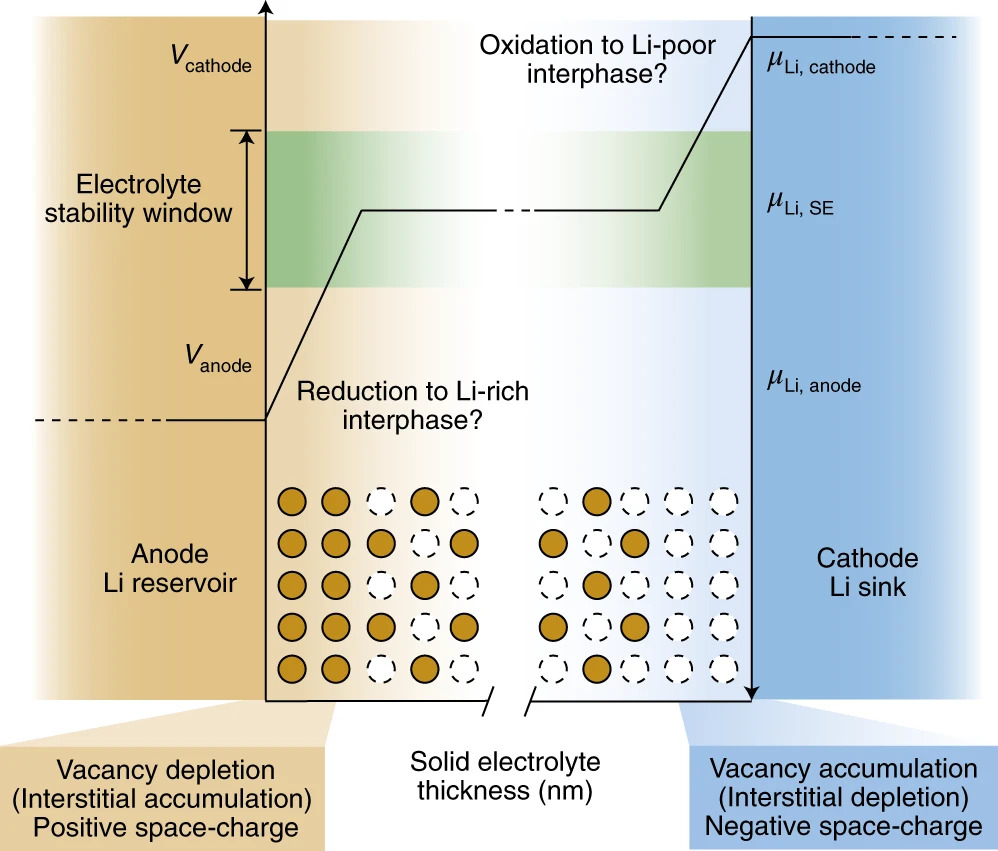
\includegraphics[width=10cm]{sestructure.jpg}
\caption{\label{sestructure.jpg} Electrochemistry of a solid state battery \cite{RN1}}
\end{figure}

It is also interesting to note that solid state electrolytes tend to have near unity lithium-ion transference number, while this number tends to be around $ 0.2-0.5 $. lithium-ion transference number is the ratio of the mobility of lithium ions to the sum of mobility of all ions. 
This means that liquid electrolytes with the same lithium conductivity will have $ 2-5 $ times higher overall conductivity. \cite{RN30}
In an ideal scenario, none of these reactions happen and the interface is intrinsically stable.
However, this is not usually the case.
In most cases, the interface needs to be stabilised.
It can be stabilised kinetically, which involves a combination of the aforementioned three reactions leading to the formation of an interphase layer at the electrode-electrolyte interface.
For kinetic stabilisation, it is important that this interphase is a good ionic conductor for the mobile charge carrier, but not a good electronic conductor.
If this is the case, interphase effectively screens the rest of the electrolyte from the electrodes, but allows the passage of the mobile ins.
The interphase reduces chemical decompositions by forming a physical barrier and it reduces redox reactions by not allowing electrons to pass into the electrolyte.
As the thickness of the interphase grows, eventually it shields the electrolyte so strongly that no more reactions can take place and so the electrode is stabilised. \cite{RN1}

If kinetic stabilisation is not possible (eg. if the interphase is electronically conductive), artificial stabilisation is required. 
This involves the artificial introduction of a performed coating layer as a buffer material. 
This can then act as the interphase that forms naturally in case of kinetic stabilisation.
Artificial interphases are typically acidic oxides, such as \ch{Li4Ti5O12}. \cite{RN77}

The major issue with electrode-SE interfaces is that they often impede the movement of the mobile ion carriers. 
In case of intrinsic stability, the “formation of lithium/sodium depleted space-charge layers due to the chemical potential difference between the SE and electrode materials” also presents a significant barrier for ion diffusion across the SE-electrode interface. \cite{RN46}
For kinetic and artificial stabilisation, the interphase formed rarely has as high conductivity as the bulk electrolyte.

Furthermore, the problem at the interfaces is not just chemical in nature.
The resistance of materials to delaminate is described by surface adhesion, an example of electrochemical coupling. 
Electromechanical coupling has contributions from the chemical interfacial energy (difference between interactions at surface and bulk), mechanical strain (lattice misfit between phases) and electrochemical attraction (charge reorganisation). 
During electrochemical reactions near the electrodes, electrochemical strain develops as the electrode undergoes cyclic expansion and contraction, which reduces the surface adhesion and can have detrimental consequences to the operation of the entire device.
Then, there are issues with keeping a good physical contact at the interface due to the stress developed on electrochemical cycling causing cracking\cite{RN44} and delamination\cite{RN45}. 
This can lead to a high level of ohmic resistance.

Indeed, there are arguments that the minimalization of interfacial impedances (both physical and electrochemical) is the key to the mass production of all-solid-state batteries, rather than the maximisation of conductivity. \cite{RN47}
This argument is based on the idea that all-solid-state batteries with reasonable energy density will be so thin that conductivity will be rarely limiting. 
It has also been argued that other than chemical, electrochemical and mechanical problems that causes problems at interfaces, there is also a more fundamental issue relating to the “differences in the way that solids and liquids screen the electric field at interfaces”. 
There has been work published about a low-capacity but high-cyclical solid-state microbattery based on Li$|$LiPON$|$\ch{LiNi_{0.5}Mn_{1.5}O4}\cite{RN48}, highlighting that there are in fact two main limiting factors for the development of all-solid-state batteries. 

\section{History of solid electrolytes}
 
Inorganic ionic conductors are not a new sensation, as they date all the way back to the early 19th century. 
The earliest examples discovered by Faraday were materials such as \ch{Ag2S} and \ch{PbF2}, both of which appeared to be conductive when heated. \cite{RN11}
The first application for these early solid-state materials was reported in the 1960s where a $ \beta $-alumina structure with mobilised sodium ions was used as a conducting medium in electric generators. \cite{RN12} 
This \ch{Na+}-$\beta$-alumina technology was further improved in the 1980s, with the introduction of the ZEBRA batteries. These batteries were the first breakthrough in making safe and corrosion-resistant batteries for commercial uses. 
The high energy density these batteries had allowed for energy-intensive applications, such as batteries for electric cars. \cite{RN13}
Initially ZEBRA-type batteries were limited to use in applications where high operating temperatures of around 250 $^{\circ}$C were tolerable, as these early solid conductors were molten-salt type batteries.
For a wider commercial use the technology needed to improve.

With progress in the field, solid-state batteries operating at ambient temperatures were developed based on lithium-ion transport in the solid state. 
These first utilised organic polymers, such as poly(ethylene) oxide\cite{RN14}, but later worked their way into inorganic solids. 
Soon, the expanding group of well-known solid electrolytes included compounds like \ch{Li3N} and \ch{Li-$\beta$’’-Al2O3}. 
While these early examples presented opportunities, they were not ideal as solid electrolytes. 
For example, \ch{Li3N} has been reported with high conductivity, but with a low decomposition voltage and extreme sensitivity towards moisture, it has limited use. \cite{RN3} 
Nevertheless, this material actually found use as a protective layer for Li anodes in liquid electrolytes. \cite{RN16}
Similarly, \ch{Li-$\beta$’’-Al2O3} also shows excellent conductivity but is also highly hygroscopic and difficult to prepare. \cite{RN17} Thus, the work to improve solid electrolyte performace continued.

\subsection{Lithium solid electrolytes}

The field of solid-state lithium ion batteries operating at ambient temperature is now growing rapidly starting with the discovery of electrolyte materials much better suited for commercial use. 
The importance of the field is also illustrated by decorated scientists, such as Nobel Prize winner John B. Goodenough contributing to the ongoing research. \cite{RN40}
Solid-state electrolytes can be divided into two main groups, oxide-based and sulfite-based ones. 

\subsubsection{Oxide-based lithium solid electrolytes}

The first group of modern solid-state were the \textbf{LiSICON} (Li Super Ion CONductors) materials, with general formula \ch{Li_{2+2$x$}Zn_{1-$x$}GeO4}, discovered in the late 1970s
They were the first example of oxide-based solid electrolytes, which is a group described by great chemical stability and relatively high ionic conductivity.
Their main drawback is processability.

Another one of the ambassadors of the ambient temperature solid-state electrolytes were lithium phosphorus oxynitride (\textbf{LiPON}) thin films. 
These materials were developed in the early 1990s.They had good conductivities for their time at around $10^{-7} \, S \, cm^{-6}$. 
However, they had issues with keeping a good contact with the electrodes and as more conductive materials were developed, they became less relevant. \cite{RN15} 

Oxide-based solid electrolytes also include \textbf{perovskite-structured} lithium lanthanum titanate (LLTO) with general formula \ch{Li_{3$x$}La_{2/3-$x$}$\square$_{1/3-2$x$}TiO3} (0.04 $<$ x $<$ 0.17). 
Developed in the early 2000s, these materials are promising with high bulk ion conductivity ($\sim 10^{-3} \, S \, cm^{-1}$), low electronic conductivity and a wide electrochemical window $(> 8 V)$. Furthermore, it was also reported great contact with the electrodes. \cite{RN18}
An issue found with this material was poor grain boundary conductivity, due to the lack of charge carrier \ch{Li+} in the grain boundary\cite{RN6}, so additives are needed to improve performance. 

Currently, the oxide-based solid electrolyte with the highest known ionic conductivity belongs to the \textbf{garnet-type} group of conductors. 
Initially, it was a group with general formula \ch{Li3Ln3Te2O12}, with Ln being Y or a member of the lanthanide group, that drew interest with a reasonably high conductivity. \cite{RN22}
Subsequently, studies found that substituting various components of this structure could lead to further enhancements in conductivity.
For example, the structure with formula \ch{Li6BaLa2Ta2O12} can have conductivity of $4 \times 10^{-5} \, S \, cm^{-1}$. \cite{RN23}
However, the most successful oxide-based garnet-type solid electrolyte is currently \ch{Li7La3Zr2O12}, which can reach conductivities over $10^{-3} \, S \, cm^{-1}$. \cite{RN85}

Another oxide-based solid electrolyte of high importance to this work is \textbf{anti-perovskite} species such as \ch{Li3OX} species. 
This will be discussed later in great detail. 



\subsubsection{Sulfide-based lithium solid electrolytes}

The other large group of solid-state conductors are sulfide-based solids.
While oxide-based electrolytes were the first ambassadors of modern solid-state conductors, generally, members of the sulphide-based group were found to have the highest conductivities.
The advantage of replacing the oxide ions in LiSICONs with the more polarizable sulphide ions is that this weakens the interactions of the anions with Li, hence leading to lower migration barriers and higher Li conductivity. 
Further, sulphide electrolytes tend to be more ductile and exhibit lower grain boundary resistance than oxides. 
Despite the high conductivity, good processability and decent chemical stability, sulfide-based conductors have not yet outcompeted oxide-based alternatives due to their poor moisture stability.

The first group of sulfide-based solid-state conductor was discovered almost two decades after the first oxide-based one in the early 2000s. 
These were the \textbf{thio-LiSICONs} (sulphide-based Li Super Ion CONductors), whose conductivity was over $10^{-3} \, S \, cm^{-1}$.
This group includes a large range of species with general formula \ch{Li_{$x$}M_{1-y}M’_{y}S4}.
The discovery of the group lead to a huge interest in these types of materials and few years later several groups of materials with even higher conductivities were reported.
 
\textbf{LGPS} with formula \ch{Li10GeP2S12} has been found to have extremely high conductivity of $1.2 \times 10^{-2} \, S \, cm^{-1}$, which is as high as that for conventional organic liquid electrolytes. \cite{RN24}
However, this type of electrolyte shows a small electrochemical window\cite{RN25} and poor stability with Li metal anode\cite{RN26}. 
Furthermore, the low abundance of Ge makes large-scale applications difficult. \cite{RN3} 
Variations upon the structure (such as LSPS-Cls like \ch{Li_{9.54}Si_{1.74}P_{1.44}S_{11.7}Cl_{0.3}}) have been investigated, but stability could not be increased without a significant drop in conductivity.  

Another promising sulphide-based solid electrolyte group is the \textbf{argyrodite-type} materials with general formula \ch{Li6PS5X}, where the partial substitution of sulphur by halogen anions stabilises a more conductive phase of the argyrodite. \cite{RN27}
There are a large range of other thiophosphates distantly related to the argyrodite material (but not quite the same structure) that have also been shown to have high conductivity. \cite{RN3}

Yet another high-conducting sulfide-based material group is \textbf{\ch{Li2S-P2S5}} materials. The front-runners from this group are \ch{Li3PS4} and \ch{Li7P3S11}.

Finally, \textbf{layered sulphides}, such as \ch{Li2SnS3} and \ch{Li2Sn2S5} represent a series of fast-conducting sulphide solid electrolytes. 
\ch{Li2SnS3} is more well-studied and has shown high conductivities albeit at high temperatures. \cite{RN28}
\ch{Li2Sn2S5} is a more Li-depleted version, giving rise more facile Li diffusion and hence a potential for higher conductivity.

\subsubsection{Polymers, phosphates, halides and hydroborates}

There are also other types of solid electrolytes worth noting. One of these are \textbf{polymer-based}. The most well-known from this group are PEO-s. 
While these types of solid electrolytes possess excellent processability and decent stability, their conductivity does not actually reach high, generally peaking at around $10^{-3} \, S \, cm^{-1}$.
Nevertheless, these types of materials found use as additives to ceramic electrolytes to improve cycling abilities.

By the early 2000s, these initial LiSICON compounds were optimised to develop \textbf{phosphate-based LiSICON-type} materials with general formula \ch{LiM2(PO4)3}. 
The tweak increased the conductivity of these compounds from around $10^{-7} \, S \, cm^{-1}$ to $10^{-4} \, S \, cm^{-1}$.
The material with Ti as "M" was found good conductivity, however, this also showed high porosity. \cite{RN19}
To overcome this issue, Ti was partially substituted with trivalent cations to make structures with formula \ch{Li_{1+$x$}R_{$x$}Ti_{2-$x$}(PO4)3} (LATP). 
These were found to have good conductivity and to be less porous and hence to possess better grain boundary conductivity. \cite{RN20}
Another option for optimising these structures is the addition of a second lithium compound, such as \ch{Li2O}. 
This acts as a flux at grain boundaries, increasing the density and hence the conductivity. \cite{RN21}
Analogues with Ge instead of Al (LAGPs) are currently one of the best oxide-based conductors. \cite{RN3}

\textbf{Halide-based} electrolytes have also been of sum interest, especially chloride- and bromide-based ones, due to the easy polarzability of these halide ions. \ch{Li2CdCl4} can reach conductivities of up to $10^{-4} \, S \, cm^{-1}$.

A more recent development has been the emergence of \textbf{hydroborate} conductors. 
There is currently much interest in this field with simple \ch{LiBH4} being modified to achieve higher conductivities.

\begin{figure}[h]
\centering
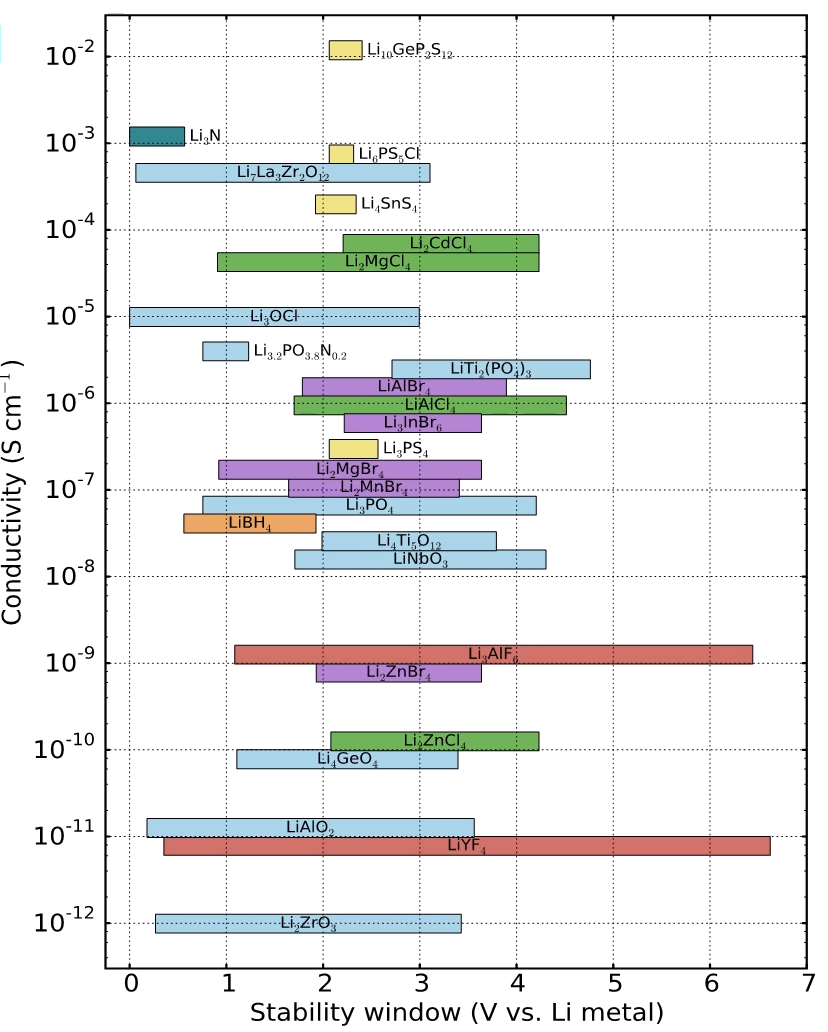
\includegraphics[width=10cm]{conductivity_vs_stability.png}
\caption{\label{conductivity_vs_stability.jpg} Conductivity and stability properties of litium solid electrolytes \cite{RN85}}
\end{figure}

\subsection{Sodium solid electrolytes}

While it was inorganic conductors with mobile \ch{Na+} charge carriers that were first discovered\cite{RN12}, it was not until more recently that the field of \ch{Na+}-based solid electrolytes began to expand. 
There has been a growing interest in the utilisation of sodium as a charge carrier in for large-scale energy storage. 
This is primarily due to their high natural abundance and so low cost. 
\ch{Na-$\beta$’’-Al2O3} is a widely used as the electrolyte in Na-S and Na-metal chloride batteries. 
At high  temperatures of 300 $^{\circ}$C its conductivity can get as high as $0.2-0.4 \, S \, cm^{-1}$. \cite{RN29} 
Other than the high operating temperatures, the high sintering temperature of this species also present issues and limits its applications. 

\subsubsection{Oxide-based sodium solid electrolytes}

NaSICON-type sodium solid electrolytes strongly resemble their lithium equivalent. 
Actually, it was NaSICON conductors that were one first discovered to have use as solid electrolytes. \cite{RN30}
Their general formula is \ch{Na_{1+$x$}Zr2Si_{$x$}P_{$3-x$}O12} $(0 \leq x \leq 3)$. 
With $ x = 2 $ conductivities of up to $6.7 \times 10^{-4} \, S \, cm^{-1}$ could be obtained at room temperature, but this can be increased to $0.2 \, S \, cm^{-1}$ at high temperatures of 300 $ ^{\circ} $C. \cite{RN31}
These materials are reported to have low thermal expansion, so operation at higher temperatures is viable.
Substitution to optimise conductivity has been researched. 
One formula that showed high conductivity was \ch{Na_{3.2}Hf2(SiO4)_{2.2}(PO4)_{0.8}}, where Zr is replaced by Hf, however, as Hf has low natural abundance, large-scale operations are not likely. \cite{RN32}
Another high-conductivity species was an Sc-doped NaSICON with a conductivity of $4.0 \times 10^{-3} \, S \, cm^{-1}$. \cite{RN33} 
Aliovalent substitution of \ch{Zr^4+} with \ch{Y^3+} was also explored and found to stabilise a higher symmetry state for the structure. \cite{RN34}
It was also proposed that modifying NaSICON with \ch{La^3+} leads to the substituted species separating out as a second phase mediating the composition of the bulk and the grain boundary. 
This would mean the grain boundary has a lessened negative effect on the conductivity, as shown by the conductivity at room temperature increasing to $3.4 \times 10^{-3} \, S \, cm^{-1}$. \cite{RN3}

Antiperovskite structures based around Na are also possible, as their lithium equivalent will be discussed later.

\subsubsection{Sulfide-based sodium solid electrolytes}

There are also sulphide-based sodium solid electrolytes, albeit much fewer types than ones involving lithium.
Furthermore, they have much lower conductivities in general. 
Sodium thiophosphates are the most well-known from this group of materials. 
The discovery of a cubic phase of \ch{Na3PS4} with conductivity of up to $4.6 \times 10^{-4} \, S \, cm^{-1}$ \cite{RN35} drew interest from a number of groups. 
It was later suggested that the high ionic conductivity was not in fact related to the crystal structure (which is actually tetragonal on a local scale), but to the defects induced during preparation. \cite{RN36}
Hence, efforts to introduce \ch{Na+} interstitials and Na vacancies have been made. 
Aliovalent doping of \ch{Si^4+} \ch{Ge^4+} and \ch{Sn^4+} for \ch{P^5+} at 6.25\% showed great improvement in conductivity with Sn being the highest, predicted at $1.07 \times 10^{-2} \, S \, cm^{-1}$. \cite{RN37}
Another strategy is the isovalent substitution of bigger ions for \ch{S^2-}. 
As mentioned before, larger ions are more polarizable and so the binding energy between them and the mobile ions will be lower, thus lowering the migration barriers. 
The highest conductivity was observed with with Se in \ch{Na3PSe4} at $1.16 \times 10^{-3} \, S \, cm^{-1}$. \cite{RN38} 

NGPSs are the equivalent of LGPSs and are another class of sulphide-based sodium solid electrolytes. 
A number of different configurations were researched, but the highest conductivity was exhibited by \ch{Na11Sn2PS12} with $1.4 \times 10^{-3} \, S \, cm^{-1}$. \cite{RN39}
It is interesting to note that in contrast with the lithium equivalent, here only octahedral sites are occupied. 

\section{Production of solid state electrolytes}

The traditional methods of synthesis of solid electrolytes can either take place via dry mixing or wet processing of reagents in a solvent.
Dry mixing requires higher temperatures, which could lead to unwanted reactions, but wet processing raises issues considering solvent recycling and waste production. 
There is also another approach involving mechanochemical synthesis, which can operate at low temperatures and require no solvent. 
However, this method appears to be problematic for scale up in terms of energy consumption and safety. 

Once the electrolyte is synthesised, it needs to be densified to minimise ohmic resistance. 
This can be done via sintering and hot or cold pressing. 
Once densified, the solid electrolyte needs to be integrated with the electrodes and the other components of the battery. 
The most popular methods for this are thin-film methods, which can achieve great solid-solid contact. \cite{RN1}

\part{Antiperovskite solid electrolytes}

\section{The antiperovskite structure}

Perovskite structures have general formula \ch{A^{2+}B^{4+}{X^{2-}}_3} are comprised of a primitive cell of A with X occupying the faces and B in the centre of the unit cell inside the X octahedron. 
Alternatively, it can be looked at as a primitive cell of B with X on the edges and A in the centre of the unit cell.
Yet another point of view is to consider the structure as a cubic close packed array of A and X with a quarter of the octahedral holes occupied by B.
This arrangement of B occupying the octahedra is rather than A is favourable, as this allows the higher charge of B to be balanced by the surrounding anions. 
This cubic structure belongs to space group 221 (Pm$\overline{3}$m). \cite{RN49} 

\begin{figure}[h]
\centering
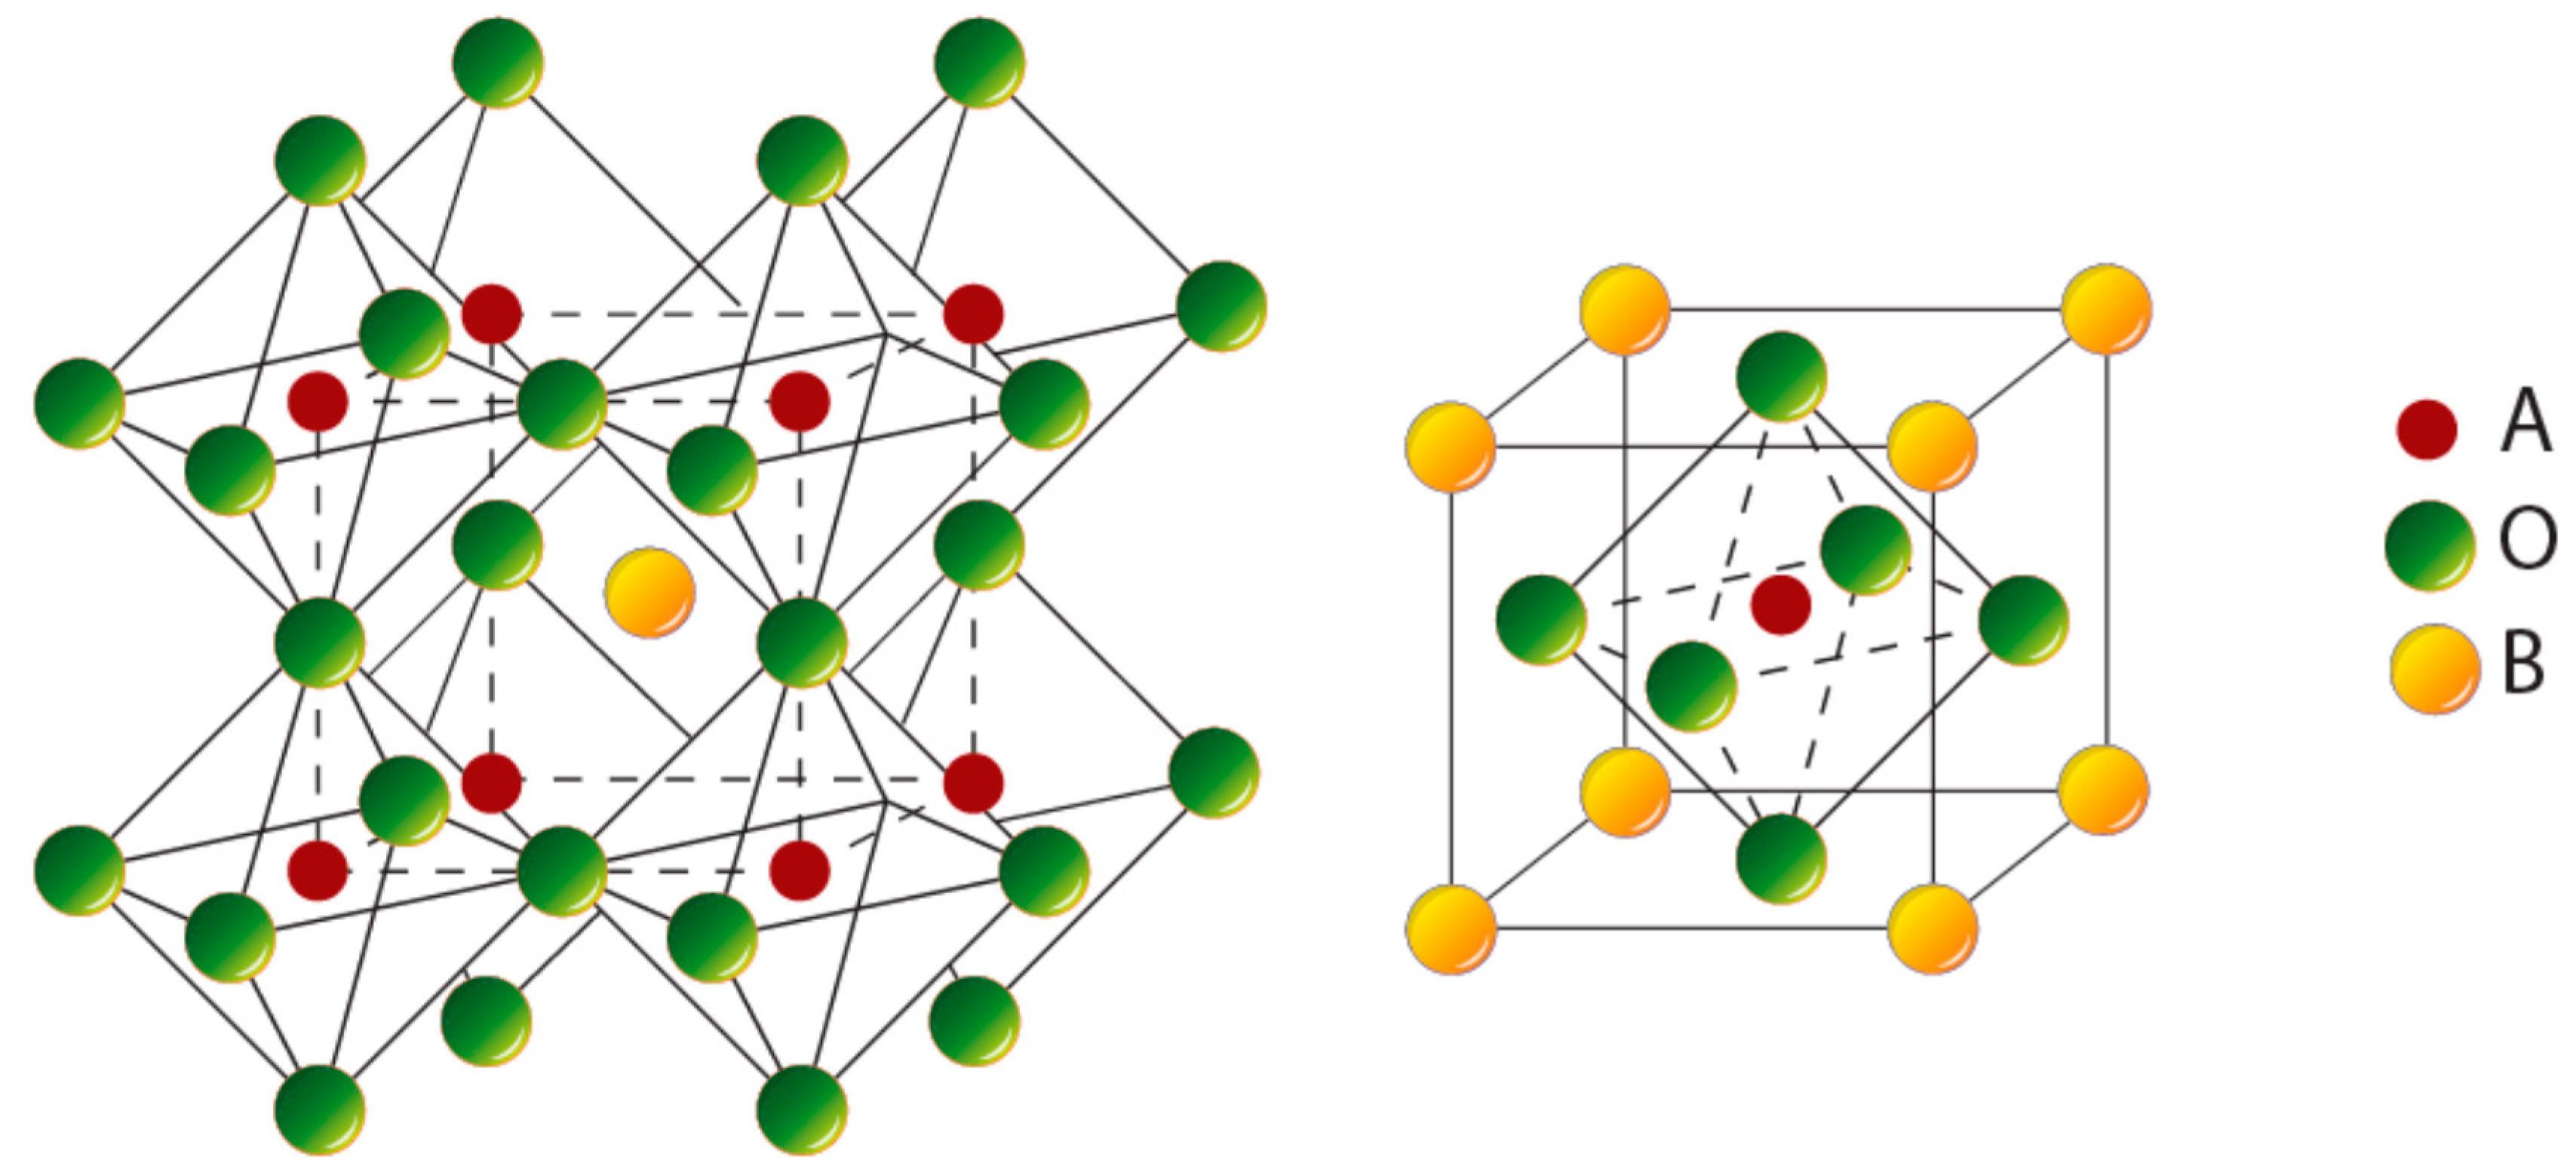
\includegraphics[width=10cm]{perovskite.png}
\caption{\label{perovskite.jpg} The perovskite structure \citep{RN50}}
\end{figure}

Anti-perovskite structures are like perovskites, but the charge of the species is different. 
They have basic formula of \ch{A^-B^{2-}{X^+}3} with B occupying the X octahedra. 
An example of this structure is \ch{Li3OCl} with O in the Li octahedra and Cl in the 12-coordinated position. 
These too were found with a cubic structure belonging to space group 221 (Pm$\overline{3}$m).

However, it is interesting to add that phonon instability in the structure is considered a limitation to the conductivity of sodium-rich antiperovskites. \cite{RN80}
One study on sodium-rich antiperovskites found that the energy of the structure can be lowered by tilting the \ch{Na6O} octahedra, making stable phonon modes more achievable. \cite{RN78}
They concluded that the P$2_1$/m phase could be more stable than the Pm$\overline{3}$m and potentially more conductive. 

Antiperovskites present several features that make them useful as solid electrolytes.
Most importantly, they possess exceptional electrochemical properties. 
A relatively high ionic conductivity, low electronic conductivity and a wide electrochemical window have all been shown to be achievable in these structures.
It was proposed these properties can be explained by the arrangement of Li ions allowing fast ion conduction. \cite{RN5}
It is interesting to note that there has been some research that suggest that body-centred-cubic-like anion network (which the anti-perovskite one could be considered) “allows \ch{Li+} ions to migrate within a network of interconnected tetrahedral sites, leading to increased conductivity". \cite{RN5}
More precisely, in a bcc anion lattice, the \ch{Li+} can move between face-sharing tetrahedral sites, which is a low barrier. 
In contrast, in case of a fcc it has to pass through an intermediate octahedral site, making the barrier higher.
Low electronic conductivity and wide electrochemical windows due to the absence of semi(metallic) elements also makes these materials and attractive alternative. \cite{RN53}
These materials are relatively soft, allowing densification, which is key for solid state batteries. \cite{RN54}

Another great advantage these materials have is being easily modified, so that ionic conductivity can be optimised with ease. \cite{RN55}
This latest property is due to the structure being prone to iso- and aliovalent substitutions. \cite{RN56}
That is the halide can be altered to larger ones and the Li can be partially substituted by divalent cations. 


\section{Lithium antiperovskite solid electrolytes}
Lithium antiperovskites have been intensively researched in the recent history, with promising results.
A relatively high ionic conductivity of $8.5 \times 10^{-5} \, S \, cm^{-1}$ has been reported meaning quick and efficient charge-discharge cycles. \cite{RN52}
Low electronic conductivity ($10^{-9}-10^{-7} \, S \, cm^{-1}$, a wide electrochemical window ($>5 V$), good thermal stability (up to 550 $K$) and stability against Li metals have also been reported. \cite{RN57}
Modification of the structure via substitutions has also lead to some early success.
For example, \ch{Li3OCl_{0.5}Br_{0.5}} was found to have a conductivity of $1.94 \times 10^{-3} \, S \, cm^{-1}$\cite{RN52}, while \ch{Li_{2.99}Ba_{0.005}ClO} was reported to have a conductivity of $2.5 \times 10^{-2} \, S \, cm^{-1}$ \cite{RN57}

It is important to note that these results have not sufficiently been back up since. 
Initial studies reported very high conductivities ($10^{-3} \,S \, cm^{-1}$)\cite{RN51, RN52}, but this value has been shown to be higher than what most subsequent studies found ($10^{-6} \, S \, cm^{-1}$). \cite{RN58}
This was proposed to be due to the presence of grain boundaries. 
These grain boundaries are generally common in \ch{Li3OCl}, as the ions have relatively low charges and so there is a low energy penalty for cleaving ionic interactions. 
It is also interesting to note that $ \Sigma $3 type boundaries tend to be lower in energy than $ \Sigma$5 types, likely due to the higher disruption in the coordination environments for the latter. \cite{RN59}  

In case of most anti-perovskite structures, the grain boundaries are more resistive than the bulk by about one order of magnitude, so the mobile ion favours the granular pathway rather than the grain boundary pathway. 
When a mobile ion moves into a grain boundary it becomes effectively trapped in the grain boundary, until it eventually escapes, when it approaches the grain with the right orientation. 
Hence, the abundance of grain boundaries restricts the mobility of the Li/Na ions and is likely to be responsible for the reduced conductivity. \cite{RN59}

Debate on the ion migration mechanism for anti-perovskite structure is ongoing. 
One of the earlier studies on the charge transport suggest that the source of the high conductivity is Frenkel defects, where the interstitial Li form a dumbbell interstitial (split interstitial), while also leaving a vacant site. 
While Frenkel type defects are quite high in energy, it was proposed that excess interstitial Li ions and/or vacancies are introduced during synthesis resulting in slight deviations from ideal \ch{Li3OCl} stoichiometry. 
Then Li migration could proceed via a coordinated three-atom move involving the dumbbell interstitial, which could be responsible for the unexpectedly high conductivity. 
However, it was also noted that the formation of interstitial defects is too high for this mechanism to fully explain the high conductivity. \cite{RN2} 

\begin{figure}
\centering
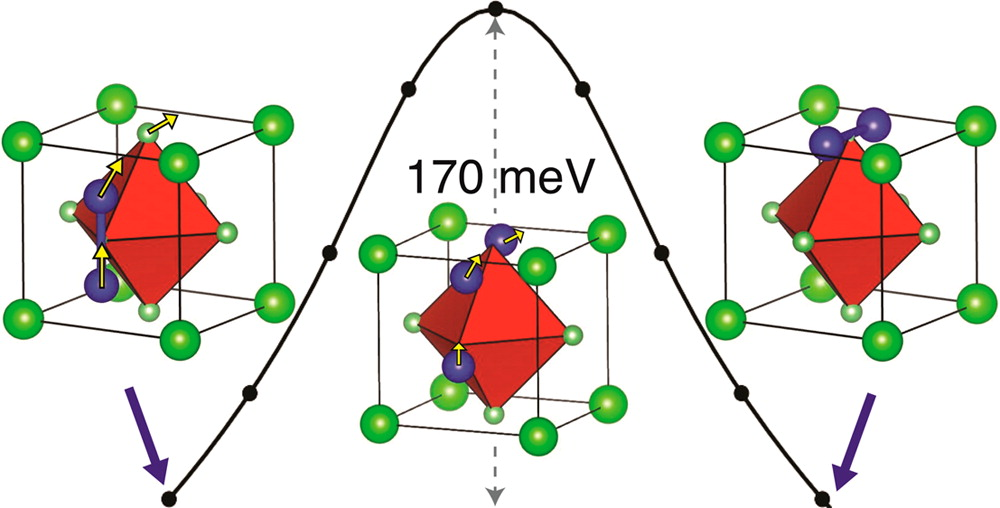
\includegraphics[width=10cm]{intmig.jpeg}
\caption{\label{intmig.jpeg} Proposed interstitial migration via the dumbell mechanism \citep{RN2}}
\end{figure}

A later study proposed that the main transport mechanism in anti-perovskites is Li/Na vacancy hopping rather than interstitial diffusion. 
They argue that Schottky vacancy defects are the dominant type of intrinsic disorder, meaning the interstitial alkali metal ion concentration is low. \cite{RN55, RN59, RN60}
More specifically, it was also proposed that the Li vacancies used for charge transport are compensated for by Cl vacancies as the NaCl partial Schottky defect is lowest in energy. \cite{RN58} 
While the second proposal is more widely accepted, the debate is yet to be settled.

The common mode of preparation for lithium-rich antiperovskites is high-temperature annealing.
Unfortunately, it was reported that preparation of \ch{Li3OCl}from dry \ch{Li2O} and LiCl is problematic and energy consuming as the reaction requires high temperatures, because of the metastable nature of \ch{Li3OCl} anti-perovskite. 
It was suggested that hydrated versions of the structure (\ch{Li_{3-$x$}OH_{$x$}Cl}) might in same cases be the product instead. 
Hydration is exothermic (-0.74 $eV$), making the reaction favourable. \cite{RN61}
They also reported that replacement of the \ch{OH-} by \ch{F-} was possible to form \ch{L2(OH)_{0.9}F_{0.1}Cl} and that this substitution results in an electrochemical window of 9 $V$ and has a stable contact with Li metal anodes. \cite{RN62}
The hydrated form takes the anti-perovskite structure at temperatures over 300 K allowing for higher ionic mobility by allowing \ch{OH-} rotation. 
The presence of \ch{OH-} rotation allows for the proton to move, allowing for easier Li hopping. \cite{RN62}
Elsewhere, it was reported that the presence of \ch{H+} allows for the formation of an amorphous glassy phase with conductivities of over $10^{-2} \, S \, cm^{-1}$. \cite{RN40, RN63}
Overall, it has been shown that the conductivities of these species are highly dependent on preparation and so it is important to find the best preparation mode. 

\section{Sodium antiperovskite solid electrolytes}

\ch{Na3NO3} (\ch{{Na^+}3{O^{2-}}NO^{2-}}) was the first sodium-rich anti-perovskite structure reported in 1938. \cite{RN64} 
However, the now well-known structures of \ch{Na3OCl} and \ch{Na3OBr} were only synthesised in 1988. \cite{RN65}
These materials were discovered to have enhanced ion transport capabilities above a transition temperature that varies from compound to compound. 
However, generally, the conductivity is too low for practical applications. 
 
At room temperature, the conductivity of \ch{Na3OX} structures vary between $10^{-10}$ and $10^{-8} \, S \, cm^{-1}$ with \ch{Na3OCl} closer to $10^{-10} \, S \, cm^{-1}$. 
As the temperature increases, so does the conductivity, with conductivity at 100 $^{\circ}C$ being between $10^{-6}$ and $10^{-8} \, S \, cm^{-1}$, with \ch{Na3OCl} at around $10^{-7} \, S \, cm^{-1}$. \cite{RN53} 
It was also reported that the value for \ch{Na3OCl} and \ch{Na3OBr} can rise to over $10^{-4}$ at 300 $^{\circ}C$. \cite{RN68} 
It is also interesting to note that one study that found \ch{Na3OBH4} has ionic conductivity in the $10^{-3} \, S \, cm^{-1}$ range at room temperature. 
The group claimed the high conductivity was due to the rotational motion of the \ch{BH4-} anion. \cite{RN70}
However, this result could not nearly be reproduced experimentally or computationally. \cite{RN53}
Another point of interest is that amorphous Na antiperovskites were resported as superionic conductors with conductivities as high as $10^{-1} \, S \, cm^{-1}$ at 150 $^{\circ}C$. \cite{RN71}

As with Li antiperovskites, it was also found that isovalent substitutions could lead to further enhancements in conductivity.
While earlier studies were somewhat sceptical on how much this strategy can improve conductivity\cite{RN55}, it was observed that at 100 $^{\circ}C$, increasing the halide size leads to an increase in conductivity. \cite{RN53} 
This is likely to be due to the increased halide size increasing the cell volume, which in turn increases the Na-O distance, which leads to weaker coordination and easier Na-ion hopping. 
Increasing the halide size also decreases the activation energy, which can be explained by the lattice becoming softer due to the more polarizable halide.
Similarly, it was suggested that replcaing the \ch{O2-} with \ch{S2-} could further enhance conductivity. \cite{RN53}

Aliovalent substitution has also been explored and perhaps offers even more possibilities to improve conductivity.
In particular the use of divalent alkaline earth metal cations appears to be especially effective.
Combining both isovalent and aliovalent doping, \ch{Na_{2.9}Sr_{0.05}OBr_{0.6}I_{0.4}} was found to have an improved conductivity of $1.9 \times 10^{-3} \, S \, cm^{-1}$. \cite{RN68}

Another interesting type of antiperovskite are inverted anti-perovskites, such as \ch{Na3FS}. 
Here the larger $2^-$ ion occupies the 12-coordinate site and the small $1^-$ ion occupies the octahedral, 6-coordinate site might also be of some interest. \cite{RN67}

While these findings are encouraging, the ion conduction mechanism in \ch{Na3OX} compounds have yet to be confirmed. 
Computational studies on \ch{Na3OCl} suggest the dominant defects are NaCl partial Schottky defects. \cite{RN55, RN72}
At the same time, it was found from neutron diffraction studies that in \ch{Na3OBr} the most common defects are \ch{Na2O} partial Schottky defects. \cite{RN66}
Nevertheless, most studies are now in agreement that the dominant \ch{Na+} defects are vacancies and hence ionic transport is via vacancy hopping.
Activation energies for these hops calculated (for \ch{Na3OCl}: 0.61 eV\cite{RN72} and 0.428 eV\cite{RN68} via DFT and 0.29 eV\cite{RN53} via MD) fall somewhat short of those measured experimentally (for \ch{Na3OCl}: 1.04 eV\cite{RN53} and 0.63 eV\cite{RN68, RN55}).

Due to the soft nature of sodium anti-perovskites, popular methods for the synthesis of sodium-rich antiperovskites begin with the high energy ball-milling of \ch{Na2O} and NaCl.
Most methods then carry on with an annealing process to increase the density of the material.
Annealing processes include hot pressing (HP), cold pressing (CP) and spark plasma splintering (SPS).
SPS is a promising technique that takes advantage of conductive graphite dies to achieve Joule heating.
The great advantage of SPS is that it makes the annealing process rapid.
It was also shown that SPS can reduce the interfacial impedance and the activation energy of the ion migration process in the solid-state electrolyte. \cite{RN79}
The formation energy for the reaction was calculated to be 72.7 $meV$/formula unit, suggesting the compound is metastable. \cite{RN72}
It was found that if the \ch{Na2O} was purified before the milling stage, there would be no need for an annealing process. \cite{RN53}
Whether annealing was applied or not during the preparation does not seem to greatly influence the ionic conductivity. \cite{RN53, RN79}
Either way, the activation energies for the Na diffusion from impedance measurements fall significantly short of those calculated, likely due to  grain boundaries, as discussed before.
It was also found that samples made via the mechanochemical route tend to have larger lattice parameters than those made by high-temperature annealing. \cite{RN53}
For \ch{Na3OCl}, lattice parameters found experimentally include 4.491 \AA\cite{RN68}, 4.496 \AA\cite{RN69}, 4.500 \AA\cite{RN65} made via high-temperature annealing and 4.504 \AA\cite{RN53} via the mechanochemical milling route. 

While synthesising sodium-rich anti-perovskite structures, it is important to keep in mind the tolerance factor for the structure. 
In the equation below, $t = 1$ corresponds to the ideal case, where ions fit perfectly in a cube. 
It was found that oxides with $0.84 < t < 0.97$ were sythesisable. 
Deviations from this can lead to phase instability and the cubic shape changing. \cite{RN53}

$$ t = \frac{r_X + r_{Na}}{\sqrt{2}(r_C + r_{Na})} $$

However, as it was found that structures with S as C could not be synthesised at all. 
Based on this and the wide range of acceptable tolerance factors for oxides, it was concluded that synthesisability is more related to the type of element occupying the octahedral sites than the tolerance factor. 
It is unclear why sulfide-based anti-perovskites cannot at this point be synthesised, but it is worth noting that oxysulfides with 30\% sulfide were successfully synthesised. \cite{RN53} 

Based on tabulated ionic radii, the expected sodium-oxygen distance is 2.34 \AA, meaning the lattice parameter of each oxide anti-perovskite should ideally be 4.68 \AA. 
However, based on experimental data, the actual value is lower than this and is a function of the halide size, with $a = 0.50 \times r_x + 3.59$. \cite{RN53}

\part{Compuational methods}

\section{Interatomic potentials}

The atomistic potential model uses empirical equations to model solid-state lattice by simulating interactions between charged ions of the lattice. 
It is also able to repeat the unit cell in all directions by applying periodic boundary conditions. 
While both the empirical equations and the periodic boundary conditions are approximations, they provide an excellent mean to run cheap calculations on lattices, which is ideal for defect calculations. \cite{RN73} 

The model uses the system’s coordinates for calculations, described by the following equation for two- and three-body systems: 

$$ U_L = \sum_{ij} V_{ij}(r_{ij}) \ + \sum_{ijk} V_{ijk}(r_{ijk}) \ + \: ... $$

These terms are comprised of long- and short-range interactions that are modelled by the Born model and interatomic potentials, respectively. 

$$ F = \frac{q_iq_j}{4\pi\varepsilon_0r_{ij}} $$

In the Born equation above, the electrostatic force between two bodies is directly proportional to the charge of the species and inversely proportional to the distance between the species. 
It is also inversely proportional to the permittivity, signified by $ \varepsilon_0 $. 
These coulombic interactions can account for as high as 90\% of the total lattice energy in ionic materials. \cite{RN74}

$$ \Phi_{ij}(r_{ij}) = A\exp\frac{-r_{ij}}{\rho_{ij}} - \frac{C_{ij}}{r_{ij}^6} $$

The equation above describes the Buckingham potential, one of the most popular interatomic potentials used to model the short-range interactions. 
A, $ \rho $ and C are parameters unique to every species. 
The positive term represents the repulsive forces of the electronic charge cloud of ions, while the negative models the attractive term. 
Interatomic potentials are most easily derived by empirical fitting to experimental data, involving the minimisation of the sum of squares.  

While the two potentials discussed describe rigid lattices well, most lattices polarisation of ions is of great importance and needs to be accounted for. 
A popular way to account for this polarisation is to apply Dick and Overhauser’s Shell Model. \cite{RN75} 
This method involves the division of each ion in the lattice into a core and a shell separated by coulombic forces. 
The core represents the nucleus of the ion and the core electrons and hence it is non-polarisable and is estimated to account for the entire mass of the ion. 
The shell is comprised of the valence electrons. so so it is polarisable and is estimated to have zero mass. 
The core and the shell have different charges, but the overall charge of the core-shell complex is equal to that of the ion. 
While the core and shell are screened by coulombic forces, they are linked via a harmonic spring, whose spring constant must also be input. 

\section{Energy minimisation}

There are a range of methods for energy minimization in computational chemistry. 
The best methods use are ones that investigate the first derivative of the potential energy function in terms of the atomic coordinates. 
These methods can find stationary points on the potential energy surface: minima and saddle-points. 
To differentiate between these two points the second derivative must be found. 
For a minimum, all second derivative must be positive.  

One method taking advantage of the derivatives of the potential energy function is the steepest descent algorithm. 
Here, the atomic coordinates are changed in a way that leads to the steepest gradient, meaning the largest decrease in energy. 
The direction in which the atomic coordinates are moved is described by the gradient unit vector ($r_i$) which points in opposite direction to the gradient vector. 
Then, the distance to be moved can be determined by either a step of an arbitrary length or a line search, though the arbitrary step method is preferred. 
This method moves the atoms by an arbitrary length ($ \alpha_i $) along the gradient unit vector. 
The method eventually converges on a minimum through a series of orthogonal successive steps. 
While this method is convenient for finding minima far from the initial starting point, it is not considered efficient. 

$$ x_{i+1} = x_i + \alpha_i r_i $$

An improvement over the steepest descent method is the conjugate gradient method. 
This algorithm uses a set of orthogonal vectors pointing in each dimension and only minimises the energy once. 
Then, the minimum is found by minimising the energy with respect to each dimension and combining these to get a search vector (di). 
Using this method has the advantage of being quicker than the steepest descent approach. 

$$ x_{i+1} = x_i + \alpha_i d_i $$

The third method is the Newton-Rapson method. 
This is a more complex method, where each new iteration is calculated by taking the atomic coordinates of the current configuration and subtracting the corresponding gradient for that point multiplied by the reciprocal of the Hessian matrix. 

$$ x_{i+1} = x_i H_{i-1}g_i $$

While the Newton-Raphson method is great at finding minima rapidly, it is less useful for finding minima that are far from the starting point. 
This is because the model relies on the potential energy surface being harmonic or near harmonic, which is true for potential wells, but not for the surface in general. 
If there is no reliable experimental data available, a combination of steepest descent or conjugate gradient and Newton-Raphson method is often applied. 

\section{Periodic boundary condiutions}

Solid lattices are theoretically infinite in all directions, meaning these systems are large. 
Modelling all of these atoms would be really expensive. Periodic boundary conditions allow this computational cost to be reduced greatly. 
This takes advantage of the regular patterns of solid lattices and the repetitive unit cells. 
In a calculation, a unit cell is modelled as being surrounded by other identical unit cells in all directions. 
Ions in the unit cell being investigated can interact with all surrounding ions, but ions in the surrounding unit cells may only interact with ions in the unit cell being investigated. 
Then, the energy of the unit cell can be calculated and scaled up to yield lattice energies. 

\section{Defect modelling}

When a defect is added to a system, the whole lattice will slightly change, especially the ions nearest to the defect. 
Therefore, it is important to include some additional relaxation effect, primarily long-range ones. 
The Mott-Littleton approximation is used for this purpose. 
This model accounts for the loss of symmetry by splitting the lattice into two regions.  

The region nearest the defect (Region I) include the defect and the ions surrounding it. 
This region of the lattice is relaxed explicitly to account for the great degree of disorder and includes both Buckingham potentials and coulombic forces. 
The outer region (Region II) then covers the rest of the lattice extending to infinity and is further divided into sub-regions IIa and IIb. 
In Region IIa, the ions in the lattice relax as a result of the ions in Region I relaxing and thus this region is modelled as a result of the central charge defect with coulombic forces exclusively. 
In Region IIb, the defect is only felt in a dielectric manner and so there is no actual displacement of ions, only a change in polarisation. \cite{RN76}

\bibliographystyle{rsc}
\bibliography{exportlist}

\end{document}